%Fred's NSF Grant Dec 2018
% GitHub: https://github.com/fjhickernell/NSF_CompMath2018Nov
% Overleaf: https://www.overleaf.com/9576964687whkhbmrrvhsd
\documentclass[11pt]{NSFamsart}
\usepackage{latexsym,amsfonts,amsmath,amsthm,epsfig,extdash,multirow}
\usepackage{stackrel,tabularx,mathtools,enumitem,xspace}
\usepackage[dvipsnames]{xcolor}
\usepackage[numbers]{natbib}
\usepackage{hyperref,accents, booktabs}
\usepackage{algorithm, algorithmicx}
\usepackage{anyfontsize}
\usepackage{cleveref}
\newcommand{\myshade}{85}
\colorlet{mylinkcolor}{violet}
\colorlet{mycitecolor}{Aquamarine}
%\colorlet{mycitecolor}{OliveGreen}
\colorlet{myurlcolor}{YellowOrange}

\hypersetup{
	linkcolor  = mylinkcolor!\myshade!black,
	citecolor  = mycitecolor!\myshade!black,
	urlcolor   = myurlcolor!\myshade!black,
	colorlinks = true,
}


% This package prints the labels in the margin
%\usepackage[notref,notcite]{showkeys}


%\pagestyle{empty}
\thispagestyle{plain}
\pagestyle{plain}

\headsep-0.6in
%\headsep-0.45in

%%list of acronyms with links
\newcommand{\QMCSoft}{\hyperlink{QMCSoftlink}{QMCSoft}\xspace}
\newcommand{\GAIL}{\hyperlink{GAILlink}{GAIL}\xspace}
\newcommand{\QMC}{\hyperlink{QMClink}{QMC}\xspace}
\newcommand{\IIDMC}{\hyperlink{IIDMClink}{IID MC}\xspace}
\newcommand{\SAMSIQMC}{\hyperlink{SAMSIlink}{SAMSI-QMC}\xspace}
\newcommand{\SciPy}{\hyperlink{SciPylink}{SciPy}\xspace}
\newcommand{\GSL}{\hyperlink{GSLlink}{GSL}\xspace}
\newcommand{\NAG}{\hyperlink{NAGlink}{NAG}\xspace}
\newcommand{\MATLAB}{\hyperlink{MATLABlink}{MATLAB}\xspace}
\newcommand{\Chebfun}{\hyperlink{Chebfunlink}{Chebfun}\xspace}
\newcommand{\Rlang}{\hyperlink{Rlink}{R}\xspace}
\newcommand{\Julia}{\hyperlink{Julialink}{Julia}\xspace}

\textwidth6.4in
\setlength{\oddsidemargin}{0in}
\setlength{\evensidemargin}{0in}
\textheight8.9in
%\textheight9.1in

\newtheorem{theorem}{theorem}


\providecommand{\FJHickernell}{Hickernell}
\newcommand{\hf}{\widehat{f}}
\newcommand{\hg}{\widehat{g}}
\newcommand{\hI}{\hat{I}}
\newcommand{\hatf}{\hat{f}}
\newcommand{\hatg}{\hat{g}}
\newcommand{\tf}{\widetilde{f}}
\newcommand{\tbf}{\tilde{\bff}}
%\DeclareMathOperator{\Pr}{\mathbb{P}}
\DeclareMathOperator{\cost}{COST}
\DeclareMathOperator{\comp}{COMP}

\DeclareMathOperator{\loss}{loss}
\DeclareMathOperator{\lof}{lof}
\DeclareMathOperator{\reg}{reg}
\DeclareMathOperator{\CV}{CV}
\DeclareMathOperator{\size}{wd}
\DeclareMathOperator{\GP}{\mathcal{G} \! \mathcal{P}}
\DeclareMathOperator{\erf}{erf}
\DeclareMathOperator*{\argmax}{arg\,max}


\newcommand{\reals}{{\mathbb{R}}}
\newcommand{\naturals}{{\mathbb{N}}}
\newcommand{\natzero}{{\mathbb{N}_0}}
\newcommand{\integers}{{\mathbb{Z}}}
\def\expect{{\mathbb{E}}}
\def\il{\left \langle}
\def\ir{\right \rangle}
\def\e{\varepsilon}
\def\g{\gamma}
\def\l{\lambda}
\def\b{\beta}
\def\a{\alpha}
\def\lall{\Lambda^{{\rm all}}}
\def\lstd{\Lambda^{{\rm std}}}

\newcommand{\vf}{\boldsymbol{f}}
\newcommand{\hV}{\widehat{V}}
\newcommand{\tV}{\widetilde{V}}
\newcommand{\fu}{\mathfrak{u}}
\newcommand{\hcut}{\mathfrak{h}}
\newcommand{\tOmega}{\widetilde{\Omega}}
\newcommand{\tvarrho}{\widetilde{\varrho}}

\newcommand{\bbE}{\mathbb{E}}
\newcommand{\tQ}{\widetilde{Q}}
\newcommand{\mA}{\mathsf{A}}
\newcommand{\mB}{\mathsf{B}}
\newcommand{\mC}{\mathsf{C}}
\newcommand{\mD}{\mathsf{D}}
\newcommand{\mG}{\mathsf{G}}
\newcommand{\mH}{\mathsf{H}}
\newcommand{\mI}{\mathsf{I}}
\newcommand{\bbK}{\mathbb{K}}
\newcommand{\mK}{\mathsf{K}}
\newcommand{\tmK}{\widetilde{\mathsf{K}}}
\newcommand{\mL}{\mathsf{L}}
\newcommand{\mM}{\mathsf{M}}
\newcommand{\mP}{\mathsf{P}}
\newcommand{\mQ}{\mathsf{Q}}
\newcommand{\mR}{\mathsf{R}}
\newcommand{\mX}{\mathsf{X}}
\newcommand{\mPhi}{\mathsf{\Phi}}
\newcommand{\mPsi}{\mathsf{\Psi}}
\newcommand{\mLambda}{\mathsf{\Lambda}}
\newcommand{\cube}{[0,1]^d}
\newcommand{\design}{\{\bx_i\}_{i=1}^n}

\DeclareMathOperator{\err}{err}
\DeclareMathOperator{\oerr}{\overline{\err}}
\DeclareMathOperator{\herr}{\widehat{\err}}
\DeclareMathOperator{\Ans}{ANS}

\DeclareMathOperator{\Var}{Var}
\DeclareMathOperator{\SOL}{SOL}
\DeclareMathOperator{\APP}{APP}
\DeclareMathOperator{\ALG}{ALG}
\DeclareMathOperator{\ERR}{ERR}
\DeclareMathOperator{\OPER}{OPER}



\DeclareMathOperator{\INT}{INT}
\DeclareMathOperator{\OPT}{MIN}

\newcommand{\bone}{\boldsymbol{1}}
\newcommand{\bzero}{\boldsymbol{0}}
\newcommand{\binf}{\boldsymbol{\infty}}
\newcommand{\ba}{{\boldsymbol{a}}}
\newcommand{\bb}{{\boldsymbol{b}}}
\newcommand{\bc}{{\boldsymbol{c}}}
\newcommand{\bd}{{\boldsymbol{d}}}
\newcommand{\be}{{\boldsymbol{e}}}
\newcommand{\bff}{{\boldsymbol{f}}}
\newcommand{\bhh}{{\boldsymbol{h}}}
\newcommand{\beps}{{\boldsymbol{\varepsilon}}}
\newcommand{\tbeps}{\tilde{\beps}}
\newcommand{\bx}{{\boldsymbol{x}}}
\newcommand{\bX}{{\boldsymbol{X}}}
\newcommand{\bh}{{\boldsymbol{h}}}
\newcommand{\bj}{{\boldsymbol{j}}}
\newcommand{\bk}{{\boldsymbol{k}}}
\newcommand{\bg}{{\boldsymbol{g}}}
\newcommand{\bn}{{\boldsymbol{n}}}
\newcommand{\bv}{{\boldsymbol{v}}}
\newcommand{\bu}{{\boldsymbol{u}}}
\newcommand{\by}{{\boldsymbol{y}}}
\newcommand{\bt}{{\boldsymbol{t}}}
\newcommand{\bz}{{\boldsymbol{z}}}
\newcommand{\bvarphi}{{\boldsymbol{\varphi}}}
\newcommand{\bgamma}{{\boldsymbol{\gamma}}}
\newcommand{\bphi}{{\boldsymbol{\phi}}}
\newcommand{\bpsi}{{\boldsymbol{\psi}}}
\newcommand{\bnu}{{\boldsymbol{\nu}}}
\newcommand{\balpha}{{\boldsymbol{\alpha}}}
\newcommand{\bbeta}{{\boldsymbol{\beta}}}
\newcommand{\bo}{{\boldsymbol{\omega}}}  %GF added
\newcommand{\newton}[2]{\left(\begin{array}{c} #1\\ #2\end{array}\right)}
\newcommand{\anor}[2]{\| #1\|_{\mu_{#2}}}
\newcommand{\satop}[2]{\stackrel{\scriptstyle{#1}}{\scriptstyle{#2}}}
\newcommand{\setu}{{\mathfrak{u}}}

\newcommand{\me}{\textup{e}}
\newcommand{\mi}{\textup{i}}
\def\d{\textup{d}}
\def\dif{\textup{d}}
\newcommand{\cc}{\mathcal{C}}
\newcommand{\cb}{\mathcal{B}}
\newcommand{\cl}{L}
\newcommand{\ct}{\mathfrak{T}}
\newcommand{\cx}{{\Omega}}
\newcommand{\cala}{{\mathcal{A}}}
\newcommand{\calc}{{\mathcal{C}}}
\newcommand{\calf}{{\mathcal{F}}}
\newcommand{\calfd}{{\calf_d}}
\newcommand{\calh}{{\mathcal{H}}}
\newcommand{\tcalh}{{\widetilde{\calh}}}
\newcommand{\calI}{{\mathcal{I}}}
\newcommand{\calhk}{\calh_d(K)}
\newcommand{\calg}{{\mathcal{G}}}
\newcommand{\calgd}{{\calg_d}}
\newcommand{\caln}{{\mathcal{N}}}
\newcommand{\cL}{\mathcal{L}}
\newcommand{\cP}{\mathcal{P}}
\newcommand{\cT}{\mathcal{T}}
\newcommand{\cK}{\mathcal{K}}
\newcommand{\fA}{\mathfrak{A}}
\newcommand{\fC}{\mathfrak{C}}
\newcommand{\fF}{\mathfrak{F}}
\newcommand{\fL}{\mathfrak{L}}
\newcommand{\fU}{\mathfrak{U}}
\newcommand{\hS}{\widehat{S}}
\DeclareMathOperator{\Prob}{\mathbb{P}}

\def\abs#1{\ensuremath{\left \lvert #1 \right \rvert}}
\newcommand{\bigabs}[1]{\ensuremath{\bigl \lvert #1 \bigr \rvert}}
\newcommand{\norm}[2][{}]{\ensuremath{\left \lVert #2 \right \rVert}_{#1}}
\newcommand{\ip}[3][{}]{\ensuremath{\left \langle #2, #3 \right \rangle_{#1}}}
\newcommand{\bignorm}[2][{}]{\ensuremath{\bigl \lVert #2 \bigr \rVert}_{#1}}
\newcommand{\calm}{{\mathfrak{M}}}
\DeclareMathOperator{\diag}{diag}
\DeclareMathOperator{\dist}{dist}
\DeclareMathOperator{\filldis}{fill}
\DeclareMathOperator{\sep}{sep}
\DeclareMathOperator{\avg}{avg}
\DeclareMathOperator{\vol}{vol}
\DeclareMathOperator{\cov}{cov}

\newcommand{\des}{\{\bx_i\}}
\newcommand{\desinf}{\{\bx_i\}_{i=1}^{\infty}}
\newcommand{\desn}{\{\bx_i\}_{i=1}^n}
\newcommand{\wts}{\{g_i\}_{i=1}^N}
\newcommand{\wtsn}{\{g_i\}_{i=1}^N}
\newcommand{\datan}{\{y_i\}_{i=1}^N}

%FJH added
\newcommand{\Order}{\mathcal{O}}
\newcommand{\ch}{\mathcal{H}}
\newcommand{\tch}{{\widetilde{\ch}}}
\newcommand{\veps}{\boldsymbol{\varepsilon}}
\DeclareMathOperator{\best}{best}
\newcommand{\hmu}{\hat{\mu}}
\newcommand{\hsigma}{\hat{\sigma}}
\newcommand{\tK}{\widetilde{K}}
%\newcommand{\Matlab}{{\sc Matlab}\xspace}
\newcommand{\abstol}{\varepsilon_{\text{a}}}
\newcommand{\reltol}{\varepsilon_{\text{r}}}

\newcommand\starred[1]{\accentset{\star}{#1}}

\newcommand{\designInf}{\{\bx_i\}_{i=1}^\infty}
\newcommand{\dataN}{\bigl\{\bigl(\bx_i,f(\bx_i)\bigr)\bigr\}_{i=1}^n}
\newcommand{\dataNp}{\bigl\{\bigl(\bx_i,f(\bx_i)\bigr)\bigr\}_{i=1}^{n'}}
\newcommand{\dataNo}{\bigl\{\bigl(\bx_i,f(\bx_i)\bigr)\bigr\}_{i=1}^{n_0}}
\newcommand{\ErrN}{\ERR\bigl(\dataN,n\bigr)}
\newcommand{\fint}{f_{\text{int}}}
\newcommand{\inflate}{\fC}


\definecolor{MATLABOrange}{rgb}{0.85,  0.325, 0.098}

%\newtheorem{resproblem}{Research Problem}
%\newtheorem{research}{Research Objectives}
%\newtheorem{keyidea}{Key Idea}
\newcounter{keyideabean}[section]
\newenvironment{keyidea}{\refstepcounter{keyideabean}\par\bigskip
   \noindent\begin{itshape}%
   Key Idea~\thekeyideabean.\ignorespaces}%
   {\end{itshape}\ignorespacesafterend}


%\setcounter{page}{1}
\usepackage{algpseudocode}
\algnewcommand\algorithmicparam{\textbf{Parameters:}}
\algnewcommand\PARAM{\item[\algorithmicparam]}
\algnewcommand\algorithmicinput{\textbf{Input:}}
\algnewcommand\INPUT{\item[\algorithmicinput]}
%\algnewcommand\STATE{\item}
\algnewcommand\RETURN{\State \textbf{Return }}


\setlist[description]{font=\normalfont\itshape}

\makeatletter
\newenvironment{varsubequations}[1]
 {%
  \addtocounter{equation}{-1}%
  \begin{subequations}
  \renewcommand{\theparentequation}{#1}%
  \def\@currentlabel{#1}%
 }
 {%
  \end{subequations}\ignorespacesafterend
 }
\makeatother


%\newcommand{\smallerscoop}{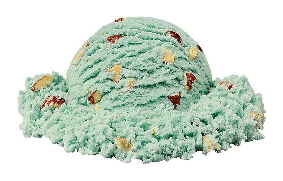
\includegraphics[width=0.7cm]{ProgramsImages/IceCreamScoop.eps}\xspace}
\newcommand{\smallerscoop}{\parbox{0.7cm}{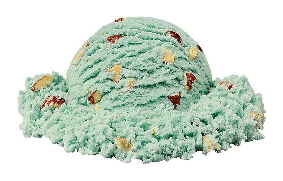
\includegraphics[width=0.7cm]{ProgramsImages/IceCreamScoop.eps}}\xspace}
\newcommand{\smallscoop}{\parbox{1cm}{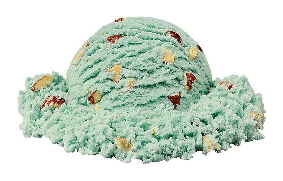
\includegraphics[width=1cm]{ProgramsImages/IceCreamScoop.eps}}\xspace}
\newcommand{\medscoop}{\parbox{1.8cm}{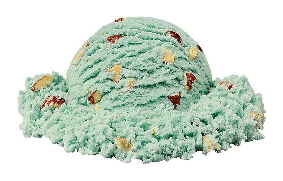
\includegraphics[width=1.8cm]{ProgramsImages/IceCreamScoop.eps}}\xspace}
\newcommand{\meddanger}{\parbox{0.8cm}{\vspace{-0.3cm}\includegraphics[width=0.75cm]{ProgramsImages/dangersign.eps}}\xspace}
\newcommand{\medcone}{\parbox{1.2cm}{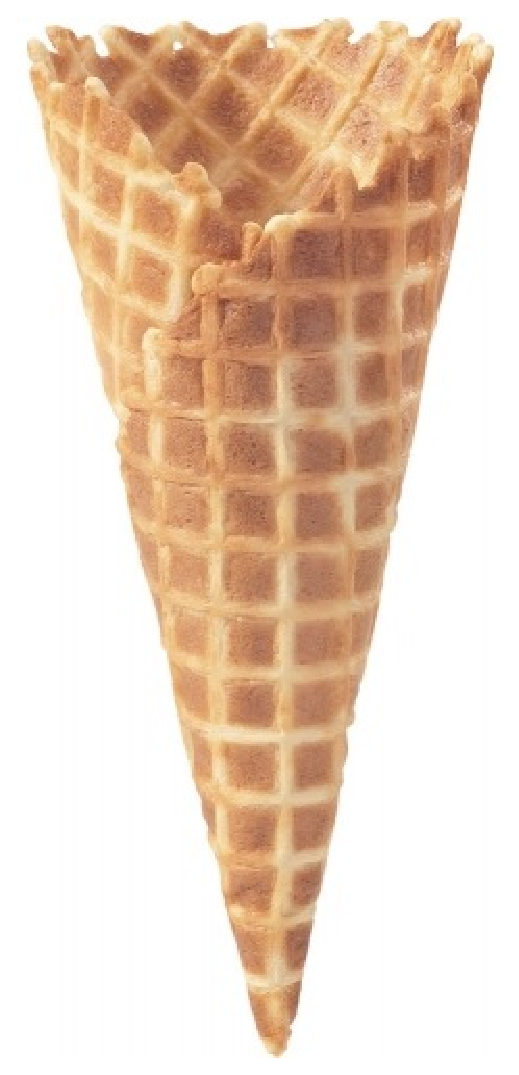
\includegraphics[width=0.55cm,angle=270]{ProgramsImages/MediumWaffleCone.eps}}\xspace}
\newcommand{\largercone}{\parbox{2.2cm}{\vspace*{-0.2cm}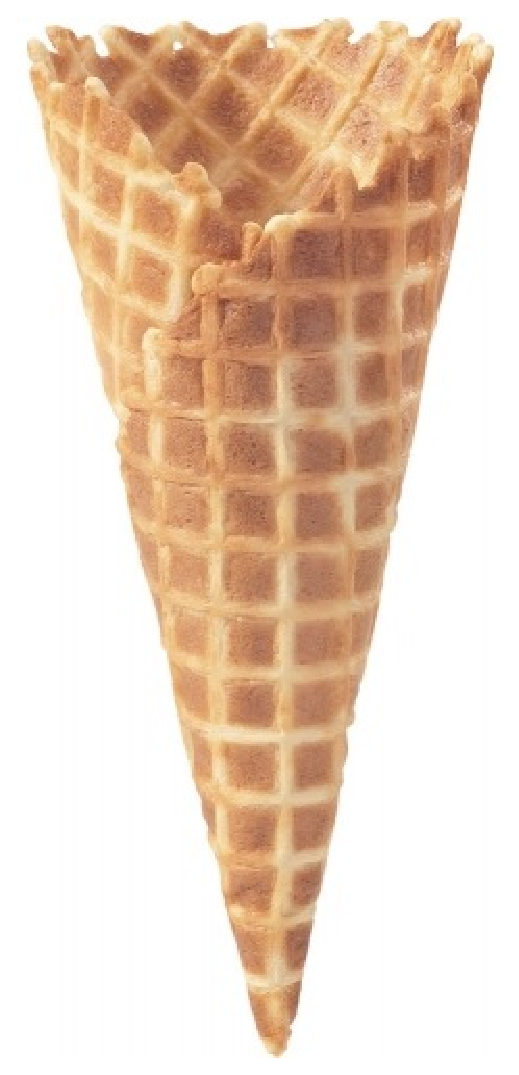
\includegraphics[width=1cm,angle=270]{ProgramsImages/MediumWaffleCone.eps}}\xspace}
\newcommand{\largecone}{\parbox{1.54cm}{\vspace*{-0.2cm}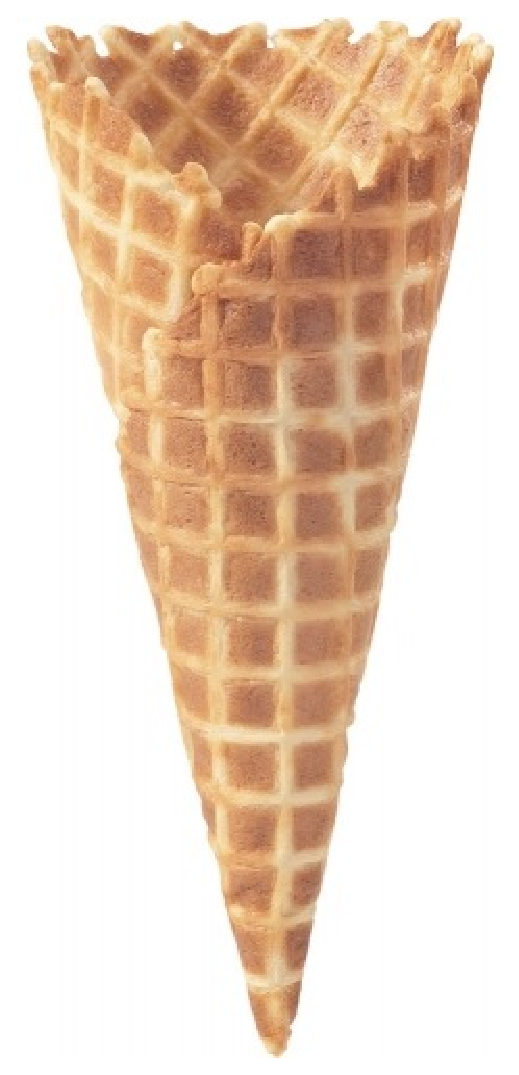
\includegraphics[width=0.7cm,angle=270]{ProgramsImages/MediumWaffleCone.eps}}\xspace}
\newcommand{\smallcone}{\parbox{0.7cm}{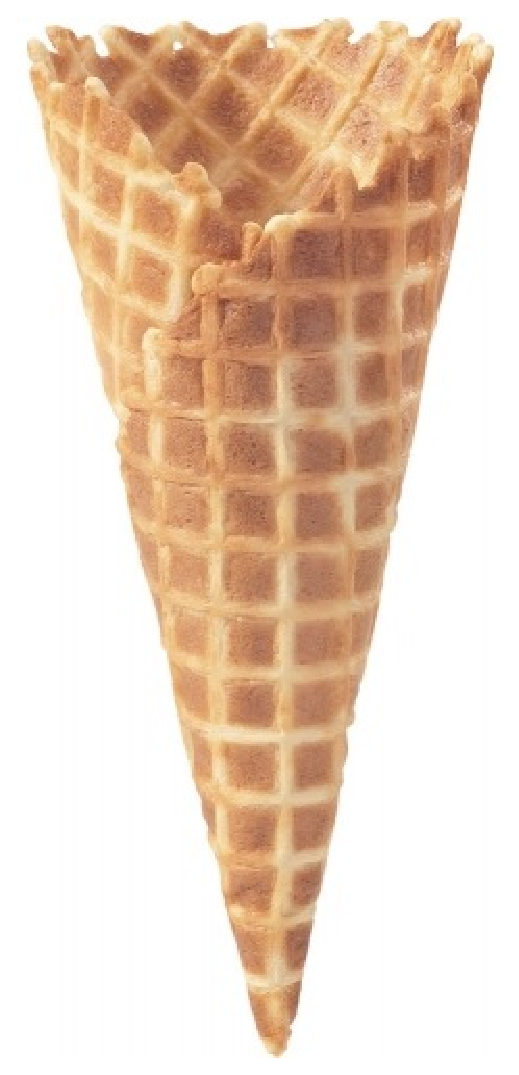
\includegraphics[width=0.32cm,angle=270]{ProgramsImages/MediumWaffleCone.eps}}\xspace}


\newcommand{\FJHNote}[1]{{\color{blue}Fred: #1}}
\newcommand{\JMHNote}[1]{{\color{green}Mac: #1}}



\begin{document}
%\setlength{\leftmargini}{2.5ex}

\begin{center}
\Large \textbf{Adaptive Sampling and Function Approximation \\ Project Description}
\end{center}
\vspace{-2ex}

\setcounter{tocdepth}{1}
\tableofcontents

\vspace{-6ex}

%%%%%%%%%%%%%%%%%%%%%%%%%%%%%%%%%%%%%%%%%%%%%%%%%%%%
\section{Scientific Context, Key Ideas, and Timeliness of the Proposed Research}
%%%%%%%%%%%%%%%%%%%%%%%%%%%%%%%%%%%%%%%%%%%%%%%%%%%%
Surrogate models are approximations of functions, $f: \Omega \subseteq \reals^d \to \reals$, that are very expensive to evaluate, e.g., the output of a complex time-consuming computer simulation.  Accurate surrogate models require a well-chosen design, $\mX_{1:n} := (\bx_1, \ldots, \bx_n)^T \in \Omega^{n} \subseteq \reals^{n \times d}$, i.e., an array of data sites where $f$ is to be evaluated.  Ideally, choice of the design should be \emph{adaptive}. The sampled function values should inform the choice of the \emph{next} data site: 
\begin{equation} \label{adaptsite}
    \bx_{n+1} = \phi_{n+1}(\mX_{1:n},\by_{1:n}), \quad \by_{1:n} := (f(\bx_1), \ldots, f(\bx_n))^T, \qquad n \in \naturals,
\end{equation}
where $\phi_{n+1} : \Omega^{n} \times \reals^n \to \Omega$ is some well chosen function that depends on underlying assumptions about $f$.  If the function is detected to be highly variable in one portion of the domain, $\Omega$, then one should place more data sites there. 

Adaptive sampling has been studied for decades.  The shortcomings of existing adaptive sampling theory are twofold:
\begin{itemize}
    \item For some adaptive sampling schemes, $\phi_{n+1}(\mX_{1:n},\by_{1:n}) = \phi_{n+1}(\mX_{1:n})$, meaning that there is no dependence on the sampled function values, $\by_{1:n}$, at all, but only on the placement of the previous data sites, $\mX_{1:n}$.
    
    \item Adaptive sampling schemes that do depend on the sampled function values are heuristic; they lack a theoretical basis.
\end{itemize}
\emph{The PIs propose to develop theoretically sound adaptive algorithms for function approximation, which adaptively choose the data sites, as in \eqref{adaptsite}, and include data-driven error bounds that can be used to stop the algorithms when the desired error tolerance is reached.}

%%%%%%%%%%%%%%%%%%%%%%%%%%%%%%%%%%%%%%%%%%%%%%%%%%%%
\subsection{Illustrative Univariate Example} 
%%%%%%%%%%%%%%%%%%%%%%%%%%%%%%%%%%%%%%%%%%%%%%%%%%%%
The univariate function $f: x \mapsto \exp(-10x) \sin(8x)$, plotted in Fig.\ \ref{fig:sampleFun}, illustrates some of the challenges of adaptive sampling.  Using the $n=10$ point design, $\mX_{1:n} = (0, 0.1, \ldots, 0.6, 0.8, 0.9, 1)^T$, an approximation, $\APP(f,n)$, is constructed as the minimum norm interpolant in the Hilbert space, $\calf$, defined by its Mat\'ern reproducing kernel,
\begin{equation}
    K(t,x) = (1 - \theta \abs{t-x}) \exp(-\theta\abs{t-x}),
\end{equation}
with $\theta = 1$.  See \cite{Buh00, Fas07a, FasMcC15a, ForFly15a, ForEtal09, SchWen06a, Wen05a} for an explanation of optimal function approximation in reproducing kernel Hilbert spaces.  The approximation is given by
\begin{equation} \label{appxExOne}
    \APP(f,n) = \sum_{i=1}^n c_i K(\cdot, x_i), \quad \text{where } \bc = \mK^{-1} \by_{1:n}, \quad \mK = \mK(\mX_{1:n}) = \bigl( K(x_i,x_j) \bigr)_{i,j=1}^n.
\end{equation}
Fig.\ \ref{fig:sampleFun} also shows $\APP(f,n)$.  

\begin{keyidea} \label{keyideainitial}
The initial design must be fill the domain well enough to detect variation in the function.
\end{keyidea}
Here, $\APP(f,n)$ captures the peak on the left because the data sites are dense enough where the peak occurs.  If the design consisted only of the $n=4$ data sites, $\mX_{1:n} = (0, 0.4,  0.6, 1)^T$, then $\APP(f,n)$ would not capture the peak.  The user might wrongly believe that the function was well approximated.  There is a substantial literature on space filling designs \cite{FangEtal19a, Jos16a, SanWilNot03}. The number of data sites required for the initial design depends on i) how many one can afford, ii) how narrow a peak one is willing to miss, and iii) the number of independent variables, $d$.

\begin{figure}[H]
    \centering
    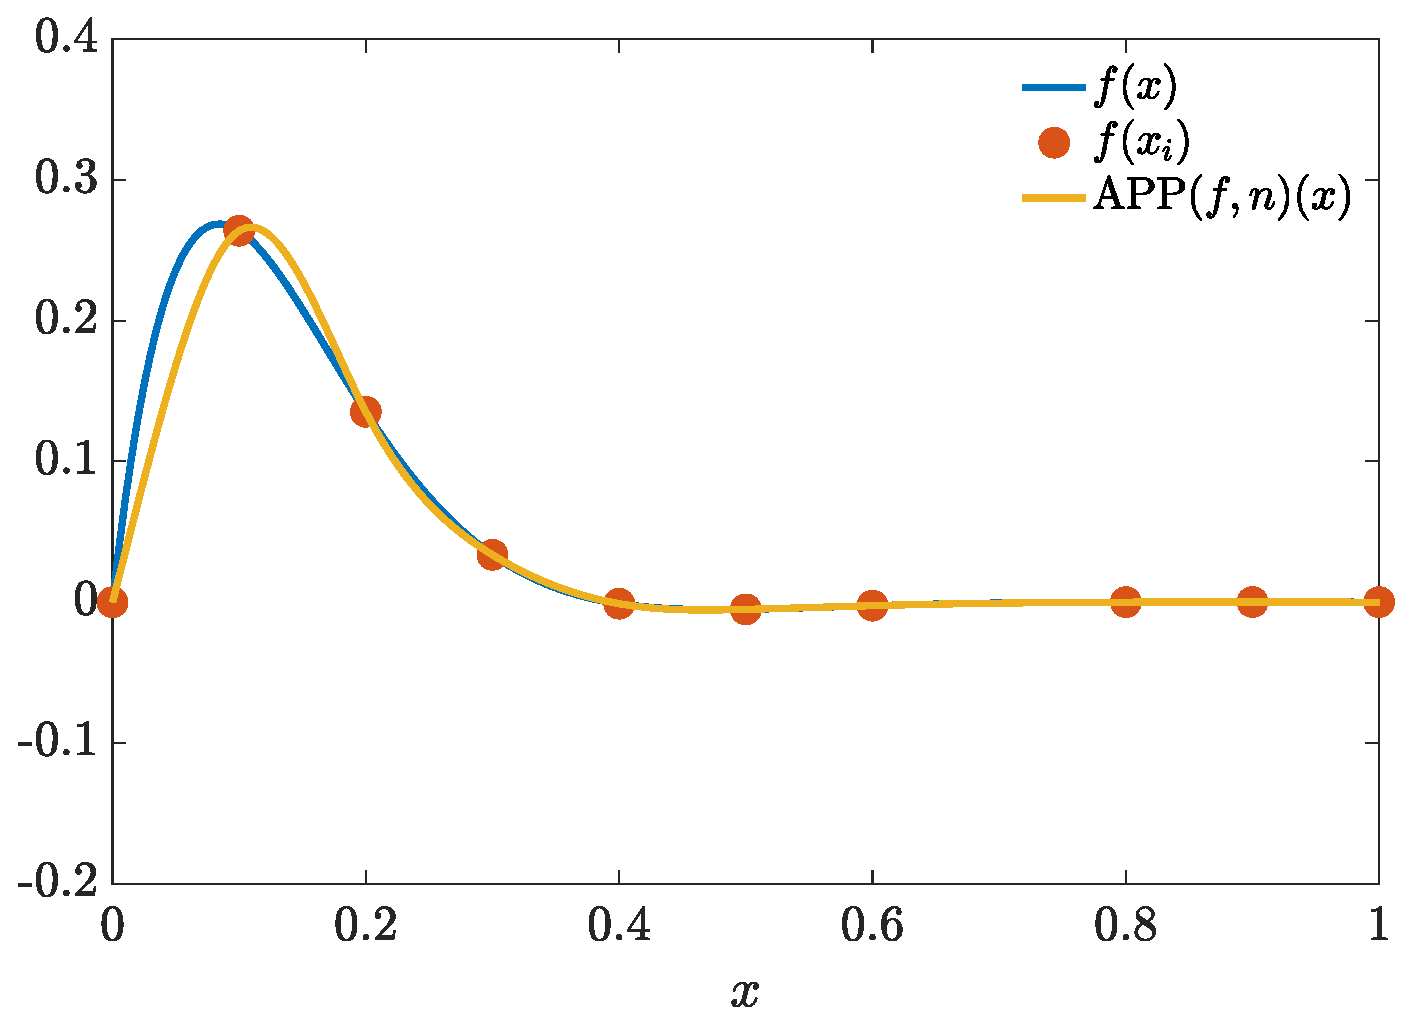
\includegraphics[width = 7cm]{ProgramsImages/fandDataAndAppx.eps} \qquad \qquad
    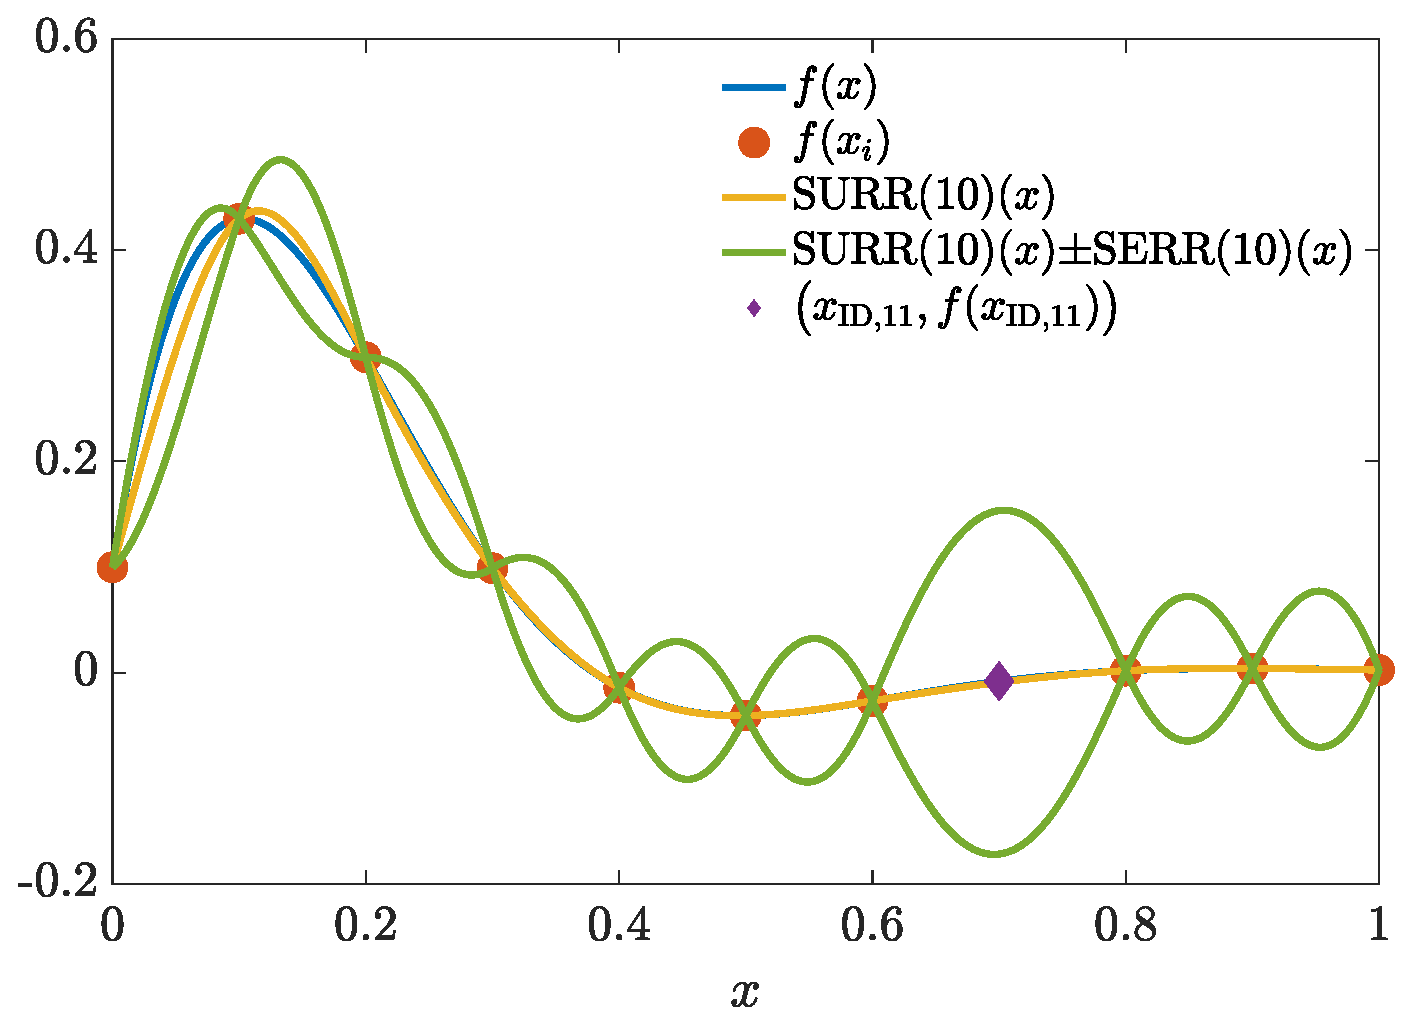
\includegraphics[width = 7cm]{ProgramsImages/fandDataAndAppxAndRMSPE.eps}
    \caption{The left plot shows $f: x \mapsto \exp(-10x) \sin(8x)$ and its approximation. The right plot also includes an approximate prediction error bound and the location of the largest prediction error, $x_{\textup{bad}}$. The largest error actually occurs far away from $x_{\textup{bad}}$.}
    \label{fig:sampleFun}
\end{figure}

Not surprisingly, the error of the approximation is greatest on the left side of $[0,1]$, where the fluctuation of $f$ is greatest.  Intuitively, one might expect that adding the next data site in the design on the left would give the greatest improvement.  Unfortunately, typical adaptive schemes do not necessarily work this way.

The approximation error has the following upper bound:
\begin{gather}
\label{RKHSErrBd}
    \abs{f(x) - \APP(f,n)(x)} \le \sqrt{K(x,x) - \bk^T(x) \mK^{-1} \bk(x)} \, \norm[\calf]{f - \APP(f,n)}, \\
    \nonumber
    \text{where} \qquad \bk(x) = \bigl(K(x,x_i) \bigr)_{i=1}^n.
\end{gather}
Choosing the next data site in the design where the approximation error is maximized corresponds to 
\begin{equation} \label{minprederr}
    x_{n+1} = x_{\textup{bad}} = \argmax_x K(x,x) - \bk^T(x) \mK^{-1} \bk(x) = \phi_{n+1}(\mX_{1:n}),
\end{equation}
which is plotted on the right in Fig.\ \ref{fig:sampleFun}.  Since the $f(x_{\textup{bad}}) \approx \APP(f,n)(x_{\textup{bad}})$, adding $x_{\textup{bad}}$ to the design does not help much.

\begin{keyidea}\label{keyideafunction}
The choice of the next data site should depend on function data, not only on the location of the other sites.
\end{keyidea}
The adaptive sampling criterion in \eqref{minprederr} does not depend at all on the function data, $\by_{1:n}$, which is why it performs poorly.  For the example in Fig.\ \ref{fig:sampleFun}, a good adaptive sampling algorithm would choose the next data site on the left where it will improve upon $\APP(f,n)$ the most.  One way to achieve this is to have the reproducing kernel, $K$, inferred from the function data, $\by_{1:n}$, in a meaningful way.  Another is to way to achieve a successful adaptive criterion is for the approximation error to be determined locally, by the nearby function data.  These approaches are elaborated in ???

As it stands, approximation error bound \eqref{RKHSErrBd} cannot be used as a stopping criterion for an adaptive function approximation algorithm because $\norm[\calf]{f - \APP(f,n)}$ is typically unknown.  However, if $n$ is large enough, we might hypothesize that our $f$ belongs to the cone
\begin{equation}
    \calc := \{f \in \calf : \norm[\calf]{f - \APP(f,n)} \le A_n \norm[\calf]{\APP(f,n)} \},
\end{equation}
where $A_n$ is positive, and fixed in advance.  This set is a cone because any multiple of an element of $\calc$ is also in $\calc$.  This $\calc$ may be interpreted as the set of functions in $\calf$ hypothesis may be interpreted as a set of functions that are not too badly approximated by $\APP(\cdot,n)$.  Since the approximation error is perpendicular to the approximation in the Hilbert space $\calf$, one may equivalently define $\calc$ as  $\{f \in \calf : \norm[\calf]{f}^2 \le (1 + A_n^2) \norm[\calf]{\APP(f,n)}^2 \}$.  Noting that $\norm[\calf]{\APP(f,n)} = \sqrt{\by_{1:n} \mK^{-1} \by_{1:n}}$ error bound \eqref{RKHSErrBd} then implies an error bound that depends completely on function data: 
\begin{equation}
\label{DataErrBd}
    \norm[\infty]{f - \APP(f,n)} \le A_n \sqrt{\norm[\infty]{K(\cdot,\cdot) - \bk^T(\cdot) \mK^{-1} \bk(\cdot)} \, [\by_{1:n} \mK^{-1} \by_{1:n}] } \qquad \forall f \in \calc.
\end{equation}
Given method for choosing data sites adaptively, an adaptive function approximation algorithm proceeds by increasing $n$ until the right hand side of \eqref{DataErrBd} does not exceed the prescribed error tolerance, $\varepsilon$.  Then the algorithm returns $\APP(f)$.

\begin{keyidea} \label{keyideacone}
Adaptive approximation algorithms are constructed for cones of functions that can be understood via a modest number of observations.
\end{keyidea}
One may

A parallel approach, which arises from Bayesian numerical analysis \cite{}, is to assume that $f$ is an instance of $\GP(0,K)$, a Gaussian process with mean zero and covariance kernel, $K$.  In this case the posterior mean of $f(x)$ given the data is the same $\APP(f,n)$ as in \eqref{appxExOne},


%%%%%%%%%%%%%%%%%%%%%%%%%%%%%%%%%%%%%%%%%%%%%%%%%%%%
\section{Results of Previous NSF-Funded Research,
NSF-DMS-1522687\except{toc}{, \\ \emph{Stable, Efficient, Adaptive Algorithms for 
Approximation and 
Integration}, \\
\$270,000, August 2015 -- July 2018}} \label{sec:Previous}
%%%%%%%%%%%%%%%%%%%%%%%%%%%%%%%%%%%%%%%%%%%%%%%%%%%%
\FJHNote{This is copied from my old proposal.  Must be revised.}

Gregory E.\ Fasshauer (GEF, co-PI) and FJH (PI) led this project.  GEF left Illinois Tech in 2016 and continued as a sub-contractor.  
SCTC contributed as senior personnel.  Other major contributors were FJH's research students Yuhan Ding (YD, PhD 2015), Lan Jiang (LJ, PhD 2016), 
Llu\'is Antoni Jim\'enez Rugama (LlAJR, PhD 2016), Da Li (DL, MS 2016), Jiazhen Liu (JL, MS 2018), Jagadeeswaran Rathinavel (JR, 
PhD student), Xin Tong (XT, MS 2014, PhD student, University of Illinois at Chicago), Kan Zhang (KZ, PhD 
student), Yizhi Zhang (YZ, PhD 2018), and Xuan Zhou (XZ, PhD 2015).  Articles, theses,  
software, and preprints supported in 
part by this 
grant 
include 
\cite{ala_augmented_2017, 
	ChoEtal17a,
	ChoEtal17b,
	Din15a, 
	DinHic20a,
	GilEtal16a,
	Hic17a,
	HicJag18b,
	HicJim16a,
	HicEtal18a,
	HicEtal17a,
	HicKriWoz19a,
	RatHic19a,
	GilJim16b,
	JimHic16a,
	JohFasHic18a,
	Li16a,
	Liu17a,
	MarEtal18a,
	mccourt_stable_2017,
	MCCEtal19a,
	mishra_hybrid_2018,
	MisEtal19a,
	rashidinia_stable_2016,
	rashidinia_stable_2018,
	Zha18a,
	Zha17a,
	Zho15a,
	ZhoHic15a}.

%%%%%%%%%%%%%%%%%%%%%%%%%%%%%%%%%%%%%%%%%%%%%%%%%%%%
\subsection{Intellectual Merit from Previous NSF Funding}
\label{previousmeritsubsec}
%%%%%%%%%%%%%%%%%%%%%%%%%%%%%%%%%%%%%%%%%%%%%%%%%%%%

%%%%%%%%%%%%%%%%%%%%%%%%%%%%%%%%%%%%%%%%%%%%%%%%%%%%
\subsubsection{Adaptive Algorithms for Univariate Problems} \label{sec:localadpat}
%%%%%%%%%%%%%%%%%%%%%%%%%%%%%%%%%%%%%%%%%%%%%%%%%%%%
In \cite{HicEtal14b}, FJH, YD, YZ, and collaborators developed an adaptive trapezoidal rule, i.e., $\SOL(f) = \int_a^b f(x) \, \dif x$.  In his PhD thesis \cite{Zha18a}, YZ constructed an improved adaptive trapezoidal rule for all integrands whose first derivatives have total variation not much greater than the total variation of their linear spline interpolant:
\[
\cc: = \left \{ f : \Var(f') \le \inflate(\size(\{x_i\}_{i=0}^n)) \Var(f'_{\textup{int},n}) \ \ \forall n \in \naturals, \ \{x_i\}_{i=0}^n), \ \size(\{x_i\}_{i=0}^n)) \le \hcut \right\}.
\]
In defining $\cc$ the nodes are arbitrary and independent of the algorithm, $\size(\cdot)$ denotes the maximum distance between adjacent nodes, $f_{\textup{int},n}$ denotes the linear spline based on $n$ nodes, and $\inflate(h) = \inflate(0) \hcut/(\hcut - h)$.  The $\ALG$ constructed by YZ  increases $n$ until the data-driven error bound does not exceed the error tolerance, following Algorithm \ref{ConeAlg}.  It satisfies  $\cost(\ALG,\cc,\varepsilon, \rho) =  \Order(\sqrt{\rho/\varepsilon})$, and is essentially optimal.  YZ also constructed an adaptive Simpson's rule.  In this case, the $f \in \cc$ have $\Var(f''')$ not much greater than the total variation of a piece-wise cubic polynomial interpolant.  Moreover,  $\cost(\ALG,\cc,\varepsilon, \rho) =  \Order([\rho/\varepsilon]^{1/4})$ and is optimal.  There is a necessary condition for $f$ to lie in $\cc$: all lower bounds on $\Var(f')$ given by $\Var(f'_{\textup{int},n})$ for various $n$ must not exceed all upper bounds on $\Var(f')$ as specified by the cone definition.

YZ's algorithms are \emph{globally adaptive}---the sampling density is constant (equally spaced nodes).  However, \emph{locally adaptive} methods (unequally spaced nodes) may perform better for univariate problems.  FJH, SCTC, YD, and XT extended the globally adaptive algorithms in \cite{HicEtal14b,Ton14a} for univariate function approximation, $\SOL(f) = f$, and minimization, $\SOL(f) = \min_{a \le x \le b} f(x)$, to locally adaptive algorithms \cite{ChoEtal17a}.  The cone $\cc$ requires $f''$ to change mildly over small intervals.  Finite differences are used to locally bound the error of the linear spline in approximating a function or seeking its minimum. Fig.\ 
\ref{localadaptfig} depicts the function data required for function approximation and minimization.  Here, $f$ is 
sampled sparsely where $|f''(x)|$ is small. For function minimization, $f$ is also sampled sparsely when $f(x)$ is significantly bigger than the observed minimum.

\begin{figure}[h]
	\centering
	\vspace{-1ex}
	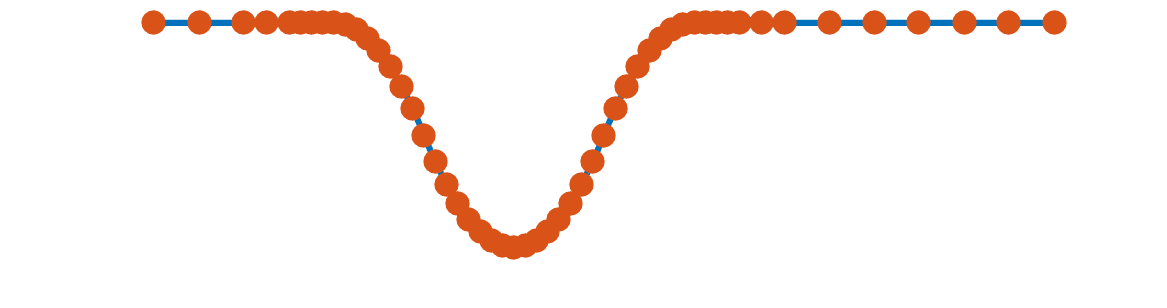
\includegraphics[width = 0.48\textwidth]{ProgramsImages/sampling-funappxg.png}
	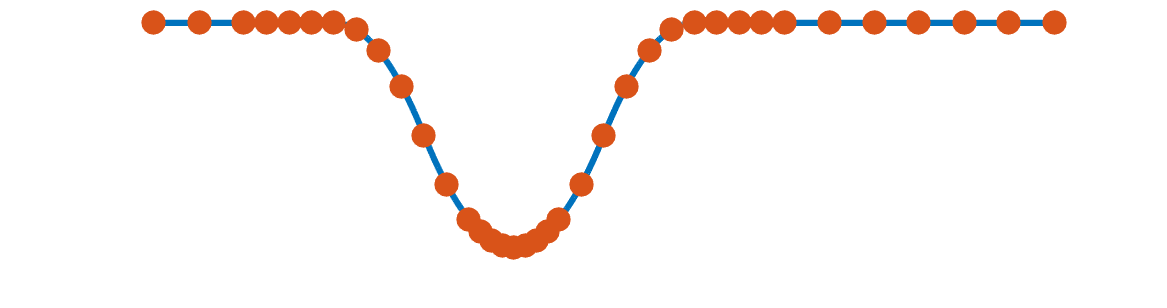
\includegraphics[width = 0.48\textwidth]{ProgramsImages/sampling-funming.png}
	
	\vspace{-2ex}
	\caption{The function data ({\color{MATLABOrange}$\bullet$}) for  locally adaptive 
	function approximation  (left) and locally adaptive optimization (right) \label{localadaptfig}}
\end{figure}


For locally adaptive function approximation algorithm 
$\cost(\ALG,f,\varepsilon) = \Order\left(\sqrt{\norm[1/2]{f''}/\varepsilon} \right)$ \cite{ChoEtal17a}.  This is essentially optimal. In contrast, 
our older globally adaptive function approximation algorithm in \cite{HicEtal14b} has a 
computational cost of $\Order\left(\sqrt{\norm[\infty]{f''}/\varepsilon} \right)$.  The local adaption algorithm may require significantly less effort because $\norm[1/2]{f''}$ may be much smaller than 
$\norm[\infty]{f''}$.

%%%%%%%%%%%%%%%%%%%%%%%%%%%%%%%%%%%%%%%%%%%%%%%%%%%%
\subsubsection[QMCsec]{Globally  Adaptive Quasi-Monte Carlo (QMC) 
Cubature} \hypertarget{QMClink}{}
\label{sec:QMC}
%%%%%%%%%%%%%%%%%%%%%%%%%%%%%%%%%%%%%%%%%%%%%%%%%%%%
FJH, LlAJR, and DL 
developed adaptive \QMC algorithms for $\SOL(f) = \int_{[0,1]^d} f(\bx) \, \dif \bx$  \cite{HicJim16a,JimHic16a}.  \QMC algorithms \cite{DicEtal14a} commonly 
choose the 
sequence of nodes, $\{\bx_i\}_{i=1}^\infty$, to be an integration lattice node sequence  or a digital
sequence, in particular, the Sobol' sequence.  \QMC cubature is superior to 
independent and identically distributed Monte Carlo (\hypertarget{IIDMClink}{IID MC}) cubature 
because the nodes are more 
evenly spread throughout the domain.   Fig.\ \ref{PtsFig} illustrates this evenness.

\begin{figure}[h] % MATLAB Driver: PlotPoints.m
	\centering
	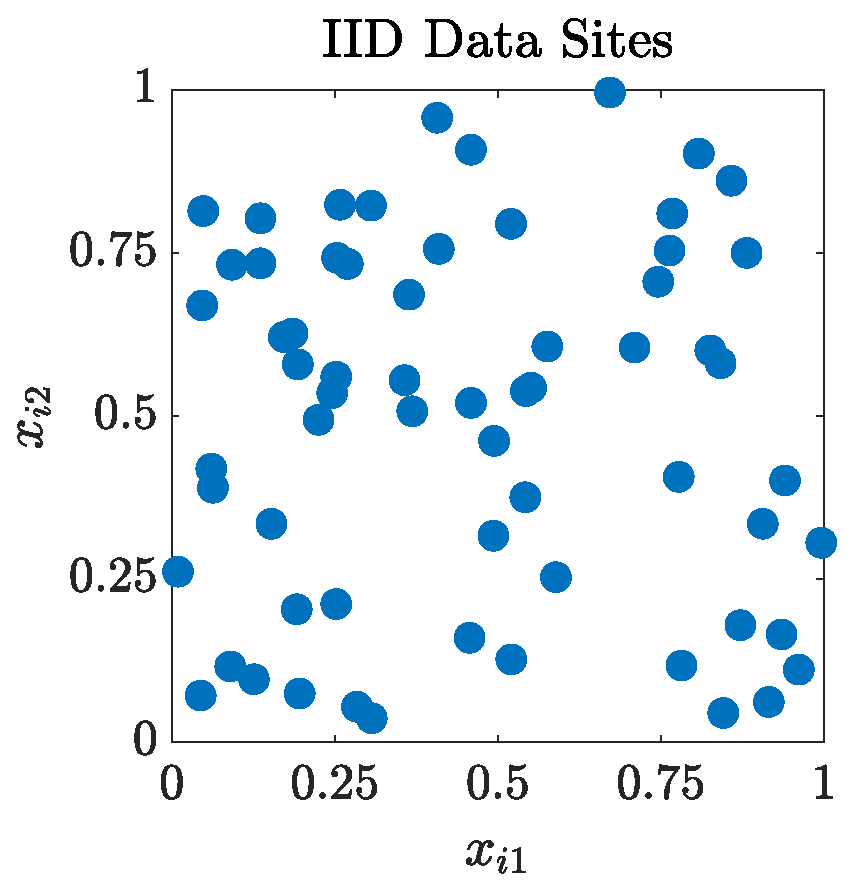
\includegraphics[width = 0.31\textwidth]{ProgramsImages/IIDPoints.eps} \quad
	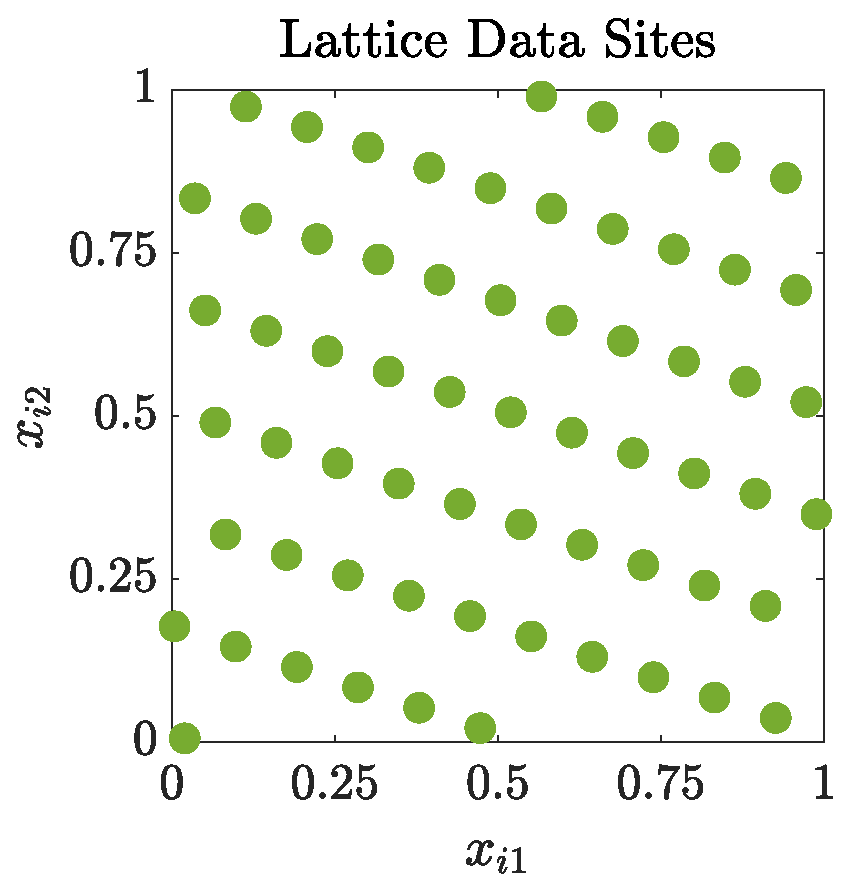
\includegraphics[width = 0.31\textwidth]{ProgramsImages/ShiftedLatticePoints.eps}  \quad
	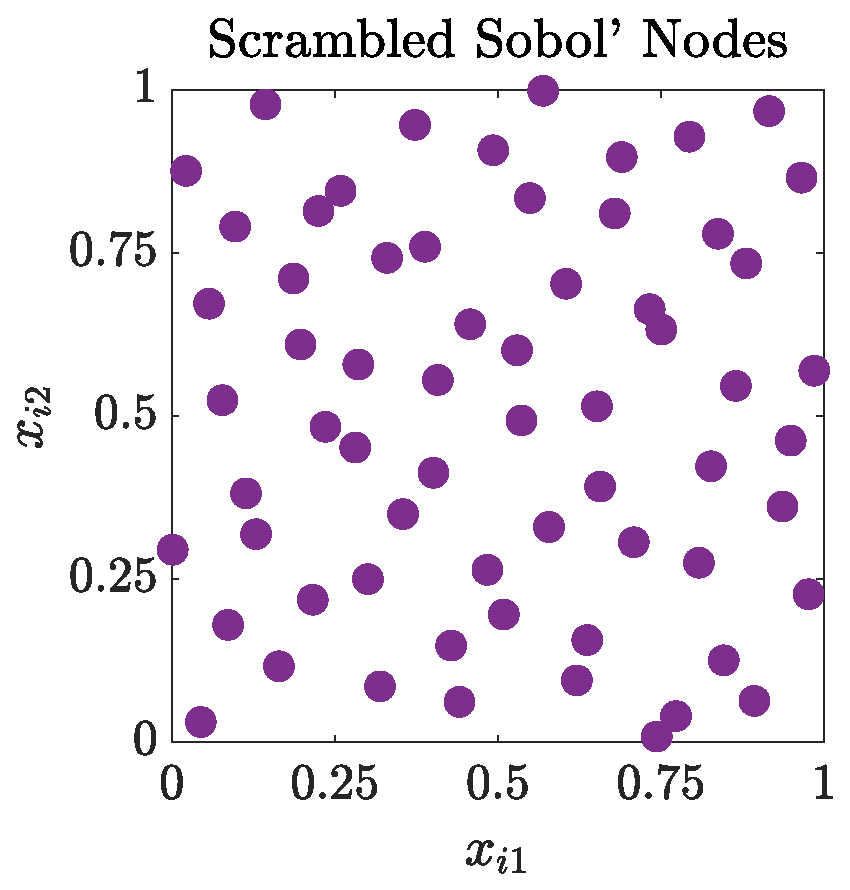
\includegraphics[width = 0.31\textwidth]{ProgramsImages/SSobolPoints.eps} 
	
	\caption{IID nodes contrasted with nodes used for QMC cubature.\label{PtsFig}}
\end{figure}

For the \QMC sampling considered here, $n$ is 
commonly a power of two.  The well-known theoretical error bound for 
\QMC cubature can be expressed in terms of some of the Fourier coefficients of the 
integrand \cite{DicEtal14a, DicPil10a, HicJim16a,JimHic16a, Nie92, SloJoe94}:
\begin{gather}
\nonumber
f(\bx) = \sum_{\bk \in \bbK} \hf(\bk) \phi_{\bk} (\bx),  \qquad \text{where } \hf(\bk) := \int_{[0,1]^d} 
f(\bx) \, \overline{\phi}_{\bk}(\bx) \quad \forall \bk \in \bbK, \\
\label{multiInt} \APP(f,n) = \frac 1n \sum_{i=1}^{n} f(\bx_i), \qquad
\abs{\SOL(f) - \APP(f,n)} \le \sum_{\bk \in P^\perp_n \setminus\{\bzero\}} \abs{\hf(\bk)} \\
\nonumber
\text{Dual set: }P_n^\perp : = \{\bk \in \bbK \, \vert \, \phi_{\bk}(\bx_i) = \phi_{\bk}(\bx_1) \text{ for } 
i=1, \ldots, n \}.
\end{gather}
For lattice nodes, $\bbK = \integers^d$ and the $\phi_{\bk}$ are complex exponentials.  For digital sequence nodes,  $\bbK = \natzero^d$ and the $\phi_{\bk}$ are Walsh functions.

FJH and LlAJR in \cite{HicJim16a,JimHic16a} defined a cone integrands, $\cc$, 
whose Fourier coefficients decay steadily, but  not necessarily monotonically.  The definition is technical, but Fig.\ \ref{GoodBadWalshFig} 
illustrates two functions and their Fourier 
(Walsh) coefficients, one inside the cone and one outside.  Here and in the error bound below, $\{\bk(\kappa)\}_{\kappa = 1}^\infty$ 
denotes an ordering of the $d$-dimensional wavenumbers in $\bbK$.

\begin{figure}[h]
	\centering
	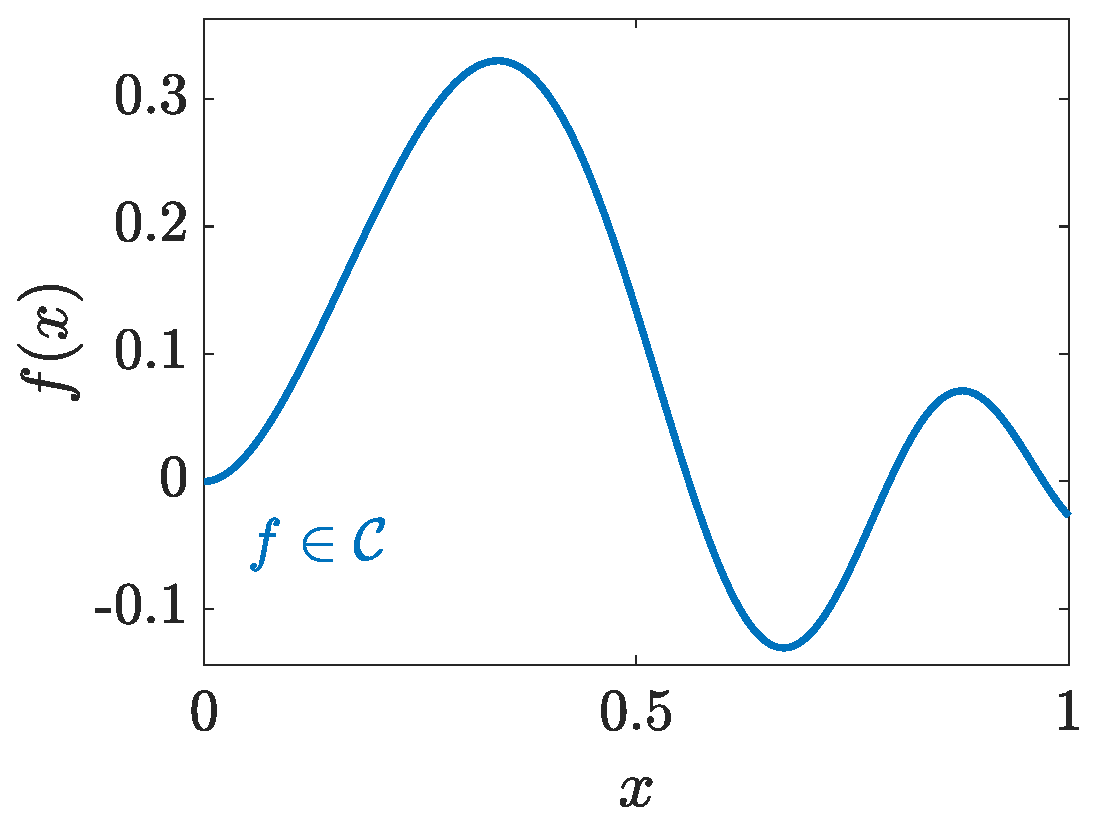
\includegraphics[width = 0.23\textwidth] 
	{ProgramsImages/FunctionWalshFourierCoeffDecay.eps} \ \ 
	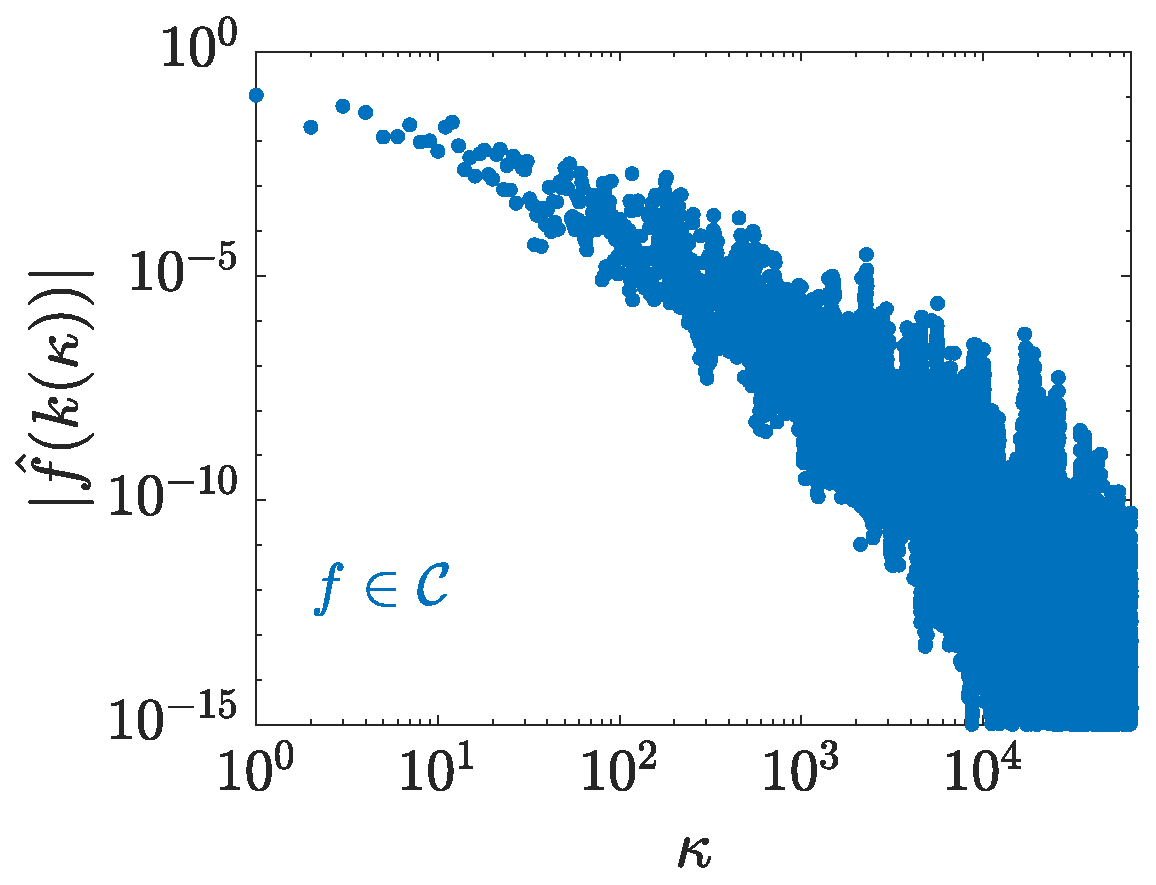
\includegraphics[width = 0.23\textwidth] 
	{ProgramsImages/WalshFourierCoeffDecay128.eps} \ \ 
	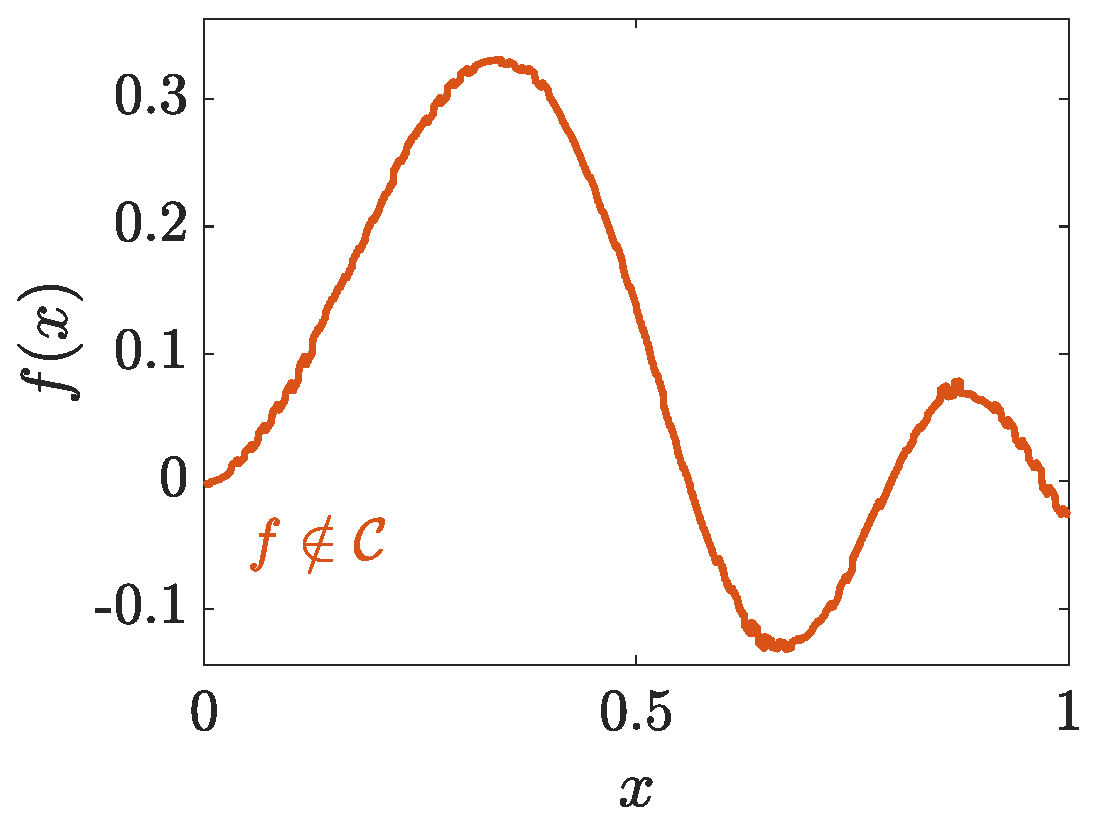
\includegraphics[width = 0.23\textwidth] 
	{ProgramsImages/FilteredFunctionWalshFourierCoeffDecay.eps} \ \ 
	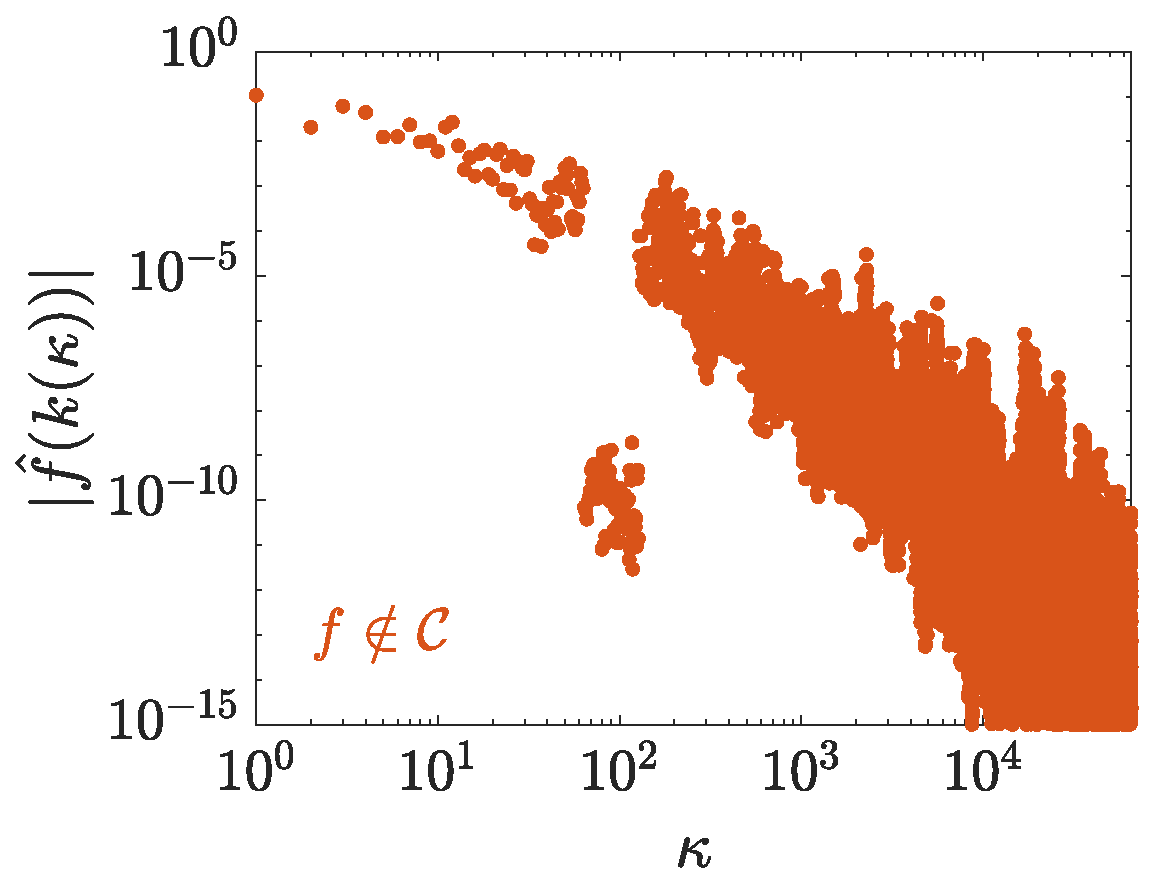
\includegraphics[width = 0.23\textwidth] 
	{ProgramsImages/WalshFourierCoeffDecayFilter.eps}
	\caption{A function inside $\cc$ and another with high frequency noise outside $\cc$
		%and their Fourier coefficients 
	\label{GoodBadWalshFig}}
\end{figure}

This definition  of $\cc$ allowed us to derive a data-driven bound on the cubature error above in \eqref{multiInt} in terms of the \emph{discrete} Fourier coefficients: 
\begin{equation*}
\ERR(\dataN,n) = \fC(n) \sum_{\kappa = n/(2n_1) + 1}^{n/n_1} \abs{\tf_n(\bk(\kappa))}, \qquad \text{where } \tf_n(\bk)  = \frac{1}n \sum_{i=1}^{n} f(\bx_i) \overline{\phi}_{\bk}(\bx_i).
\end{equation*}
Here $\fC(n)$ is an inflation factor.  The data driven error bound depends on moderate-sized wavenumbers because they best emulate the error---which comes from large wavenumbers---but their discrete Fourier coefficients are not contaminated by aliasing. This data-driven error bound is used to construct guaranteed adaptive \QMC cubature 
algorithms: $n$ is increased by doubling until $\ERR(\dataN,n^*) \le \varepsilon$.  Then choosing 
$\ALG(f,\varepsilon) = \APP(f,n^*)$ satisfies 
\eqref{AlgErr}.  As in the cases of the univariate algorithms in Sect.\ \ref{sec:localadpat}, necessary conditions for $f$ to lie in $\calc$ arise from the cone definition.  Moreover, this algorithm automatically senses the speed at which the Fourier coefficients and converges accordingly; it is smoothness adaptable.

Using a fast transform to compute the discrete Fourier coefficients, the total cost is $\Order\bigl(\$_d(f)n^* + n^* \log(n^*)\bigr)$.  So, the cost of manipulating the function data is not much worse than the computational cost of collecting the function data, a concern raised in Sect.\ \ref{sec:CompEff}.

FJH, LlAJR, and DL generalized the adaptive \QMC rules to accommodate control variates \cite{HicEtal17a}.  We also extended adaptive cubatures to a more general error criterion.  Bayesian inference \cite{GelEtal13} and computing Sobol' indices \cite{Sal02a} involve a function of \emph{more than one} integral. We vectorized the solution operator, $\SOL : \calf^p \to \reals^p$, defined the answer as some function of this vector of integrals, $\Ans: \reals^p \to \reals$, allowed a relative error tolerance, $\reltol$, and constructed an $\ALG$ satisfying
\begin{multline}
\label{generrorcrit} \tag{G-ALG-CRIT}
\abs{\Ans(\SOL(\vf)) - \ALG(\vf,\varepsilon, \reltol) } \le \max(\varepsilon, \reltol \abs{\Ans(\SOL(\vf))} ) \\
\forall \vf \in \cc^p, \ \varepsilon > 0, \ 0 < \reltol < 1 .
\end{multline}
JL derived a similar generalization for an adaptive trapezoidal rule \cite{Liu17a}.


%%%%%%%%%%%%%%%%%%%%%%%%%%%%%%%%%%%%%%%%%%%%%%%%%%%%
\subsubsection{Adaptive Bayesian Cubature}  \label{sec:Bayes} 
%%%%%%%%%%%%%%%%%%%%%%%%%%%%%%%%%%%%%%%%%%%%%%%%%%%%
The research above assumes a deterministic integrand, but recent research by FJH and JR assumes that the integrand is an instance of a Gaussian process with constant mean $m$, and covariance kernel, $C:[0,1]^d \times [0,1]^d \to \reals$, i.e., 
$f \sim \GP (m,C)$.  This \href{http://www.probabilistic-numerics.org}{probabilistic numerics} approach dates back at least thirty years \cite{Dia88a, OHa91a, RasGha03a, Rit00a} and has generated recent interest. One constructs a credible interval in the Bayesian sense, $\Prob\bigl[\abs{\SOL(f) 
- \APP(f,n)} \le \ErrN \bigr] = 99\%$, where $\APP(f,n)$ is the posterior mean.  By increasing $n$ until the width of the credible interval is no greater than the error tolerance, one has an adaptive Bayesian cubature.  The hyper-parameters, $m$ and the parameters defining the covariance kernel, $C$, may be treated by empirical Bayes (maximum likelihood estimation), full Bayes, and/or cross-validation \cite{RatHic19a}.  Although similar computations can done assuming $C$ to be a reproducing kernel for a Hilbert space, the Gaussian process approach facilitates data-driven error bounds.

A longstanding drawback of Bayesian cubature has been the computational cost of operations
involving the Gram matrix $\mC = \bigl(C(\bx_i,\bx_j)\bigr)_{i,j=1}^n$, which is ordinarily
$\Order(n^3)$.  Attempts to overcome this cost include \cite{AniCheSte16a, ParEtal17a}.  FJH and JR chose shift-invariant covariance kernels, which matched the lattice nodes used for sampling the integrand \cite{RatHic19a}. This yields Gram matrices $\mC$ for which the necessary vector-matrix operations can be accomplished by fast transforms with computational cost $\Order(n 
\log(n))$, making Bayesian cubature practical.  We also found a way to avoid the round-off error that often plagues these Gaussian process methods for large $n$.

The following table shows the performance of our adaptive cubatures in approximating the integral corresponding to the price of Asian arithmetic mean call option where the price is $\$13.12$ and $d=12$.  The cubatures were run under different scramblings of the nodes.
\[
\begin{array}{cccccr@{.}l}
    \text{Error} & & \text{Median} & & \text{Worst }10\% & \multicolumn{2}{c}{\text{Worst }10\%}\\
    \text{Tolerance} & \text{Method} & \text{Error} & \text{Success} & n & \multicolumn{2}{c}{\text{Time (sec)}} \\
    \toprule
     1\text{E}-2& \text{IID Monte Carlo \cite{HicEtal14a}} & 2\text{E}-3 & 100\% & 6.1\text{E}7 & 33\\
     1\text{E}-2&  \text{Lattice Nodes \cite{JimHic16a}} & 1\text{E}-3 & 100\% & 1.6\text{E}4 & 0&041\\
     1\text{E}-2& \text{Sobol' Nodes \cite{HicJim16a}} & 1\text{E}-3 & 100\% & 1.6\text{E}4 & 0&040\\
     1\text{E}-2&  \text{Sobol' Nodes w/ Control Variates \cite{HicEtal18a}} & 2\text{E}-3 & 100\% & 4.1\text{E}3 & 0&019\\
     1\text{E}-2& \text{Bayesian w/ Lattice Nodes \cite{RatHic19a}} & 2\text{E}-3 & 99\% & 1.6\text{E}4 & 0&051\\
\end{array}
\]

%%%%%%%%%%%%%%%%%%%%%%%%%%%%%%%%%%%%%%%%%%%%%%%%%%%%
\subsubsection{Multivariate Function Approximation} \label{sec:PrevFunAppx}
%%%%%%%%%%%%%%%%%%%%%%%%%%%%%%%%%%%%%%%%%%%%%%%%%%%%

GEF has led the effort in accurate, well-conditioned function approximation and solution of 
differential equations using reproducing kernel Hilbert space methods.  Much of his effort has been 
developing truncated Hilbert-Schmidt decomposition of the reproducing kernels using appropriate 
eigenfunctions.  For example, an expansion of the squared exponential (Gaussian) kernel using 
Chebyshev polynomials instead of Hermite polynomials has been used for the numerical solution of 
nonlinear unsteady 
convection-diffusion-reaction equations.  GEF and his collaborators extended
decompositions of the Matern kernels on the half line to the entire real line, the first such analytical 
derivations.

FJH, YD, and LlAJR investigated the solution of general linear operators, $\SOL$, when series coefficients are available \cite{DinHic20a}.  Suppose that 
\begin{subequations} \label{serForm}
\begin{gather}
    \calf := \left \{ \sum_{\bk \in \caln} \hf(\bk) u_{\bk} : \norm[\calf]{f} := \norm[r]{\left(\frac{\bigabs{\hf(\bk)}}{\lambda_{\bk}} \right)_{\bk \in \caln}} \right \},  \quad
    \calg : = \biggl \{ \sum_{\bk \in \caln} \hg(\bk) v_{\bk} : \norm[\calg]{g} := \bignorm[r']{\hg}\biggr \}, \\ 
    v_{\bk} = \SOL(u_{\bk}), \quad
     \lambda_{\bk_1} \ge \lambda_{\bk_2} \ge \cdots, \qquad
      n_0 < n_1 < n_2 < \cdots, \quad r^{-1} + r'{}^{-1} = 1.
\end{gather}

\end{subequations}
By assuming a steady decay of the series coefficients, ordered according to the $\lambda_{\bk}$, and for the case $r=2$, we constructed an adaptive algorithm defined on a cone, $\cc \subset \calf$, and based on sampling \emph{Fourier coefficients}, not function values.  This algorithm is essentially optimal.


%%%%%%%%%%%%%%%%%%%%%%%%%%%%%%%%%%%%%%%%%%%%%%%%%%%%
\subsection{Broader Impacts from Previous NSF Funding} \label{prevBIsect}
%%%%%%%%%%%%%%%%%%%%%%%%%%%%%%%%%%%%%%%%%%%%%%%%%%%%

\emph{Publications, Conference Participation, and Conference Organization.} Publications by GEF, FJH,  SCTC, students, and collaborators are listed at the beginning of this section.  We have spoken at many applied mathematics, statistics, 
and computational science conferences and given colloquium/seminar talks to mathematics and 
statistics departments.  Here are highlights.  FJH, SCTC, LJ, and LlAJR published  an 
encyclopedia entry on adaptive Monte Carlo \cite{HicEtal18a}.  FJH co-organized the 
\href{http://cos.iit.edu/2016-spring-research-conference/}{2016 Spring Research 
Conference}, a long-running annual industrial statistics conference.   FJH gave an invited tutorial 
at the \href{http://mcqmc2016.stanford.edu}{MCQMC 2016} 
\cite{Hic17a}, a biennial conference for which he serves on the steering committee.  FJH 
was a program leader for the SAMSI 2017--18 
\href{https://www.samsi.info/programs-and-activities/year-long-research-programs/2017-18-program-quasi-monte-carlo-high-dimensional-sampling-methods-applied-mathematics-qmc/
}{\QMC Program (\hypertarget{SAMSIlink}{SAMSI-QMC})}.   He  gave an invited tutorial 
	at the Opening Workshop, and led one of 
	the working groups.  FJH received the 2016 Joseph F.\ Traub 
	Prize for Achievement in Information-Based Complexity.
	
	
FJH's leadership in the MCQMC conferences  and \SAMSIQMC brought \QMC to other areas of potential application.  One concrete example, is the 
	collaboration between FJH, LlAJR and French collaborators working in uncertainty quantification \cite{GilEtal16a, GilJim16b}.  Another example, is the collaboration of LlAJR with
	high energy physicists at Fermilab, in the Chicago suburbs, using \QMC to speed 
	up their calculations.
	
\emph{\GAIL Software.} The results of this research have been implemented in 
\GAIL, our open source \MATLAB library hosted on
\href{http://gailgithub.github.io/GAIL_Dev/} {Github}. This software 
has been implemented with input parsing, input validation, unit tests, inline documentation, and 
demonstrations.  \GAIL makes it easier for practitioners to try our new adaptive algorithms.  SCTC has been key in this effort.  
%With the help of students, we are starting to port GAIL to Python and \Rlang.

\emph{Boosting the STEM Workforce.} GEF, FJH, and SCTC have mentored a number of 
research students associated with this project.  The main ones are mentioned at the beginning of 
this section.  Female students mentored include YD, LJ, JL, XT, and Xiaoyang Zhao (MS 2017).   GEF, FJH,  and SCTC have mentored many undergraduate students including more than a dozen 
Brazilian Science Mobility Program students in the summers of 2015 and 2016, Noah Grudowski (BS student IIT), Cu Hauw Hung (BS Biola U, now MS student at UCLA), Tanner Johnson (BS U Minnesota, now MS student at U British Columbia), Yueyi Li (female, BS Macalester U, now MS student at Johns Hopkins), Tianpei Qian (BS NUS, now MS student at Stanford), Alexsei Sorokin (BS student IIT), Paul Wolfert (BS student Colorado Schoo of Mines), and 
Tianci Zhu (female, now MS student at NYU).  We have also had a few high school students join us. As part of our team, all of
these students have learned how to conduct theoretical and/or practical computational mathematics research.

FJH has taught a course on Monte Carlo methods each fall.  For the past several years students 
have been introduced to \GAIL and used it in their coursework.  \GAIL has been used to teach how 
to know how large $n$ must be for an \IIDMC or \QMC simulation to reach the desired accuracy 
requirement.  A number of student class projects have been devoted to improving \GAIL.

In recognition of his research leadership, FJH was appointed the director of Illinois Tech's new Center for Interdisciplinary 
Scientific Computation in 2017.  In this position he fostered collaborative scientific computation 
research across departments by hosting matchmaking seminars and sponsoring a seed grant 
competition. In 2018, FJH was appointed Vice Provost for Research.




%%%%%%%%%%%%%%%%%%%%%%%%%%%%%%%%%%%%%%%%%%%%%%%%%%%%
\section{Intellectual Merit of the Proposed Research} \label{sec:Proposed}
%%%%%%%%%%%%%%%%%%%%%%%%%%%%%%%%%%%%%%%%%%%%%%%%%%%%




%%%%%%%%%%%%%%%%%%%%%%%%%%%%%%%%%%%%%%%%%%%%%%%%%%%%
\section{Broader Impacts of the Proposed Research}\label{SectBroad}
%%%%%%%%%%%%%%%%%%%%%%%%%%%%%%%%%%%%%%%%%%%%%%%%%%%%
\FJHNote{This is copied from my old proposal.  Must be revised.}


%%%%%%%%%%%%%%%%%%%%%%%%%%%%%%%%%%%%%%%%%%%%%%%%%%%%
\subsection{Contributions to Training, Mentoring and Other Human Resource Developments}
%%%%%%%%%%%%%%%%%%%%%%%%%%%%%%%%%%%%%%%%%%%%%%%%%%%%
FJH leads a weekly research group meeting comprised of long-term and short-term student 
collaborators, visitors, the curious, and special guests.  Ongoing work in early or polished stages is shared.  Papers of other authors are presented.  Mentoring takes place during these meetings as well as individually.

\emph{Providing Research Experiences for Undergraduate and High School Students.} Students 
should be introduced to research before graduate school so that they can learn how to 
discover the unknown, something that is not necessarily taught in the classroom. We request funds 
to 
support two summer undergraduate students per year.  Our small summer research program has established some visibility 
and is prompting inquiries from prospective participants well before we 
even announce our latest 
offerings. As in the past, we expect the NSF funds will serve as a catalyst for funds to 
support additional summer students. In choosing summer students we will make a deliberate effort to 
build 
a diverse research environment by targeting female and underrepresented minority students as well 
as students from less research-focused institutions (see Sect.~\ref{prevBIsect}). We will also 
welcome well-prepared high school students to join our research group.

\emph{Preparing Students for Academic Careers.} Mentoring is a multi-faceted and 
potentially long-term process continuing even after the mentee has moved on from Illinois Tech.  
Our PhD students gain experience both research and mentoring the younger students in our 
research group.  We 
continue contact with many of our former students.  In particular we continue to 
collaborate with YD and Yiou Li (female).  We will continue to help our students prepare for 
academic careers and continue mentoring them after they leave Illinois Tech.

\emph{Preparing Students for Industry Careers.}
We also help current students land 
competitive jobs in the business world. Our training in the areas of computation and software 
development gives our students the needed edge in comparison to other mathematics 
graduates. For example, LlAJR and XZ are working in the financial services industry and  LJ is 
working in marketing analytics.  All of them are developing and testing quantitatively sophisticated 
and computationally intensive models.  LlAJR and LJ continue to collaborate with us on research.

\emph{Supervising Visitors.}
Both FJH and SCTC have strong connections to East Asia.  We have hosted several long-term 
self-funded visitors in the past and plan to do so in the future.

\emph{Giving Tutorials and Invited Lectures.}
We will continue providing lectures to students at various stages in their careers, ranging from high
school to graduate school. These encourage students to enter STEM and encourage STEM students 
to engage in research in general, and this research area in particular.


%%%%%%%%%%%%%%%%%%%%%%%%%%%%%%%%%%%%%%%%%%%%%%%%%%%%
\subsection{Contributions to Resources in Research, Education and the Broader Society} 
\label{BroaderTwoSec}
%%%%%%%%%%%%%%%%%%%%%%%%%%%%%%%%%%%%%%%%%%%%%%%%%%%%

The proposed research straddles mathematics, statistics, theoretical computer science, and 
application areas.  The two PIs have complementary strengths that facilitate this interdisciplinary research.  FJH 
has expertise in \QMC methods, kernel-based methods, information-based complexity 
theory, tractability, and experimental design. SCTC has expertise in computer science and applications.  Our 
expertise provides both an obligation and an opportunity to interact with a number of diverse 
communities. We envision the following contributions:

\emph{Disseminating Research}
The research supported by this grant will result in publications in peer-reviewed journals in applied
mathematics, computer science, statistics, and science/engineering. These 
journals will include both those that emphasize theory and those that emphasize applications.

\emph{Promoting Cones.} The idea of guaranteed, adaptive algorithms via cones of reasonable input 
functions has broad potential application.  We will continue to promote this idea among numerical analysts 
who 
develop new algorithms and analyze their computational costs, as well as among information-based 
complexity theorists who analyze the lower bounds on the complexity of numerical problems.  The recent work by Kunsch, Novak, and Rudolf \cite{KunEtal19a} shows that the idea of cones is catching on.

\emph{Bridging Applied Mathematics and Statistics.}
This project touches on topics that are of interest to the statistics community: kriging, Monte Carlo methods, probabilistic numerics, and design of experiments.  We have and will continue to engage the statistics community 
by speaking a their conferences and departmental colloquia.

\emph{Organizing and Presenting at Conferences.}
We and our students involved in this project will present our results at a variety of conferences and workshops.  These include: (i) specialized meetings focusing on approximation theory, complexity, 
experimental design, Monte Carlo methods, and probabilistic numerics; (ii) the national meetings of AMS, SIAM, and the 
statistical societies; and (iii) conferences devoted to application areas.  We are frequently invited to 
speak at such conferences, which will give our results a prominent hearing. We will also continue to 
organize specialized conferences or minisymposia within larger conferences.

\emph{Writing Survey Papers.}
FJH and SCTC will continue their practice of writing tutorial, survey, and encyclopedia articles.  These will make our findings accessible to a wider audience.

\iffalse
\emph{Refreshing Course Syllabi.}
MATH 565 (Monte Carlo Methods in Finance), taught every fall by FJH, has incorporated our new
results on guaranteed (quasi-)Monte Carlo multivariate integration. In the future it will include our 
new results on our guaranteed MLM and MDM (see Sect.\ \ref{SectMultiProb}).

As noted in Sect.\ \ref{TrapIllSect}, current texts propagate poor practices for 
adaptive quadrature.  We will urge numerical analysis textbook authors and educators to change the 
way that error estimation is taught based on our recent and proposed work.  These ideas will also 
enter our more traditional numerical analysis courses such as MATH 350 (Intro to Computational 
Math).  SCTC and FJH will continue to develop MATH 573 (Reliable Mathematical Software) as a 
valuable course for our own students and an example that we wish to propagate to other 
universities.
\fi

\emph{Creating Software and Collaborating with Software Developers.}
As the complexity of large scale numerical computations increase rapidly, mundane operations such as integration and function approximation are taken for granted. We must construct reliable adaptive algorithms for these problems so that there are no unwelcome surprises for the practitioner when she takes them for granted.

We will continue to develop \GAIL \citep{ChoEtal17b} (now up to version 2.2).  The \GAIL software 
will serve the wider community that relies on numerical approximation and integration algorithms.  It will 
also demonstrate how adaptive algorithms ought to be implemented, which we hope will inspire and 
inform those working on adaptive algorithms for other mathematical problems.  We will involve 
students in porting \GAIL to other platforms, such as Python, \Rlang, and \Julia.  

In the summer of 2018, we began engaging with other \QMC research groups about combining our software efforts.  These included the groups of Mike Giles (Oxford, Multi-Level Monte Carlo),  Frances Kuo (UNSW, \QMC generators, PDEs with random coefficients),  Dirk Nuyens (KU Leuven, \QMC generators, PDEs with random coefficients), and Christoph Schwab (ETH-Zurich, PDEs with random coefficients).  All of these groups have significant software development efforts, but our software libraries are not compatible with one another.  We have begun discussing a common framework for a shared community quasi-Monte Carlo software library, \QMCSoft.  If all groups would write their software to the specifications of this framework, then improvements and additions would immediately work with the other parts of the library.

We will collaborate with these other research groups to move our software to this common framework.  Given the difficulty in agreeing upon one language, this may be a multi-language effort.  We will seek resources outside this proposal to support this effort.  As the \QMC community embraces \QMCSoft, we expect our core of contributors to grow.  Scholars who develop new \QMC algorithms or use \QMC in applications will be encouraged to add them to \QMCSoft.  

We expect our new algorithms to be incorporated into widely used numerical packages, as was done for our algorithm in \cite{HonHic00a} by \MATLAB and \NAG.  We have already and will continue 
to discuss with software developers about good practices for adaptive algorithms.


\emph{New Applications of \QMC.}
The application of \QMC has focused on a few areas, such as financial modeling and computer 
graphics, but there is potential for much wider application.  LlAJR has collaborated with Fermilab implementing \QMC algorithms, and we plan to continue.    New applications of \QMC are arising from \SAMSIQMC that we plan to pursue.  KZ is exploring how to use adaptive \QMC to more efficiently perform Bayesian inference.


\newpage
\clearpage
%\pagenumbering{arabic}
\setcounter{page}{1}

\bibliographystyle{spbasic.bst}


{\renewcommand\addcontentsline[3]{} 
\renewcommand{\refname}{{\Large\textbf{References Cited}}}                   %%
\renewcommand{\bibliofont}{\normalsize}

\bibliography{FJH23,FJHown23}}
\end{document}


